Завершаем рассмотрение реверсивных преобразователей.
\subsection{Функциональная схема раздельного управления}
\begin{circuitikz}
  \draw[thick,dashed,double,->](0,0)--(2,0);
  \draw[thick,dashed,double,->](0,0)--(0,2)
        node[midway,left]{$U_\textcyrillic{ЗНТ}$};

  \draw
  (2,-0.5) rectangle (3.5,0.5) (2.75,0)node{БРУ}
  (-1,2) rectangle (1,3) (0,2.5)node {САР} (0,3.5)node{(ACP)}
  (1.5,1)rectangle(2.5,5) (2,3)node{ВУ}
  (4,1.5)rectangle(5.5,2.5) (4.75,2)node{СУ2}
  (4,4)rectangle(5.5,5) (4.75,4.5)node{СУ1};
%  \draw[->] (4.75,1)--(4.75,1.5);
%  \draw[->] (4.75,3.5)--(4.75,4);
  \draw[->] (2.5,2)--(4,2)node[midway,above]{$U_\textcyrillic{упр2}$};
  \draw[->] (2.5,4.5)--(4,4.5)node[midway,above]{$U_\textcyrillic{упр1}$};
  \draw[->] (3.5,0)--(3.75,0)--(3.75,3.25)--
  (4.75,3.25)node[midway,above]{$u_1$}--(4.75,4);
  \draw[->] (3.5,0)--(3.75,0)--(4.75,0)node[midway,above]{$u_2$}--(4.75,1.5);
  \draw[->,dashed] (5.5,4.5)--(7,4.5)node[midway,above]{$\alpha_1$}; 
  \draw[->,dashed] (5.5,2)--(9.5,2)--(9.5,4.5)--(11,4.5)node[midway,above]{$\alpha_2$};
  \draw[->] (1,2.5)--(1.5 ,2.5);
  % выпрямитель-инвертор
  \draw
  (7,4)rectangle(9,5)
  (7,5)node[above]{ВГ1}
  (8.5,4.5)to[Do](7.5,4.5)--(8.5,4.5)
  (7.87,4.34)--(7.70,4.17)
  (11,4)rectangle(13,5)
  (13,5)node[above]{ВГ2}
  (12.5,4.5)to[Do](11.5,4.5)--(12.5,4.5)
  (11.87,4.34)--(11.70,4.17)
  %соединения от выпрямителя-инвертора
  
  (7.5,4)--(7.5,1.5)to[L](7.5,0)
  to[american controlled current source,l=$\textcyrillic{ДТ}_1$](10,0)
  to[american controlled current source,l=$\textcyrillic{ДТ}_2$](12.5,0)  
  (8.5,4)--(8.5,3.5)--(11.5,3.5)--(11.5,4)
  (12.5,4)--(12.5,1.5)to[L](12.5,0)
  (8,5)--(8,5.5) -- (10-0.433*21/12,6.65-21/12*0.25)
  (8,5.8)node[above]{m фаз}
  (12,5)--(12,5.5)--(10+0.433*21/12,6.65-21/12*0.25)
  (12,5.8)node[above]{m фаз}
  (10,6.65+0.82)to[ospst,l_=QF](10,8.7)--++(-3,0) % к трехфазной сети
  (8,8.5)--(8.4,8.9)
  (7.8,8.5)--(8.2,8.9)
  (7.6,8.5)--(8.0,8.9)
  %мотор  (10,3.5)--(10,1.5)to[short](10,0) (10,1.25)node[component]{M}
  (10,3.5)to[short,*-](10,1.5)to[motor,-*](10,0);
  \draw[dotted](7.5,0.75)circle(0.5); % выбрасываем L уравнительный
  \draw[thin](7,0.25)--(8,1.25);
  \draw[dotted](12.5,0.75)circle(0.5); % выбрасываем L уравнительный
  \draw[thin](12,0.25)--(13,1.25);
  \draw[->] (8.75,-0.3)--(8.75,-0.75)--(3,-0.75)--(3,-0.5);
  \draw[->] (11.25,-0.3)--(11.25,-1)--(2.5,-1)--(2.5,-0.5);
  %трансформатор (10, 6.65) (-0.433,-0.25)
  \draw({10-0.433*2/3},{6.65-0.25*2/3}) circle(0.5)
  ({10+0.433*2/3},{6.65-0.25*2/3}) circle(0.5)
  (10,{6.65+0.5*2/3}) circle(0.5) 
  ;\end{circuitikz}

Трансформатор имеет особенность преобразовывать число фаз. У Каждой вентильной группы ({\it ВГ}) своя
система управления СИФУ ({\it СУ}) или система управления вентилями ({\it СУВ}).
Каждая ${\textcyrillic{\it СУ}}_N$ генерирует
сигналы с углом $\alpha_N$.
Импульсов должно быть {\it m}. Уравнительные реакторы используются только в случае совместного управления.
На схеме уравнительные реакторы обведены кружками, чтобы подчеркнуть, что в раздельном управлении они не
обязательны. При совместном управлении должно выполнятся условие $\alpha_1+\alpha_2>\pi$, в противном
случае протекает большой уравнительный ток.

\begin{circuitikz}
  \draw (4,1.5)rectangle(5.5,2.5) (4.75,2)node{СУ2};
  \draw[red,<-] (4.75,1.5)--(4.75,1) node[right,color=black]{-- вход для выключения СИФУ.};
\end{circuitikz}

\begin{circuitikz}
  \draw
  (2,-0.5) rectangle (3.5,0.5) (2.75,0)node{БРУ};
  \draw[<-] (2.2,-0.5)--(2.2,-1) node[below]{$\textcyrillic{ДТ}_1$};
  \draw[<-] (3.3,-0.5)--(3.3,-1) node[below]{$\textcyrillic{ДТ}_2$};
  \draw[dashed,double,->] (0,0)--(2,0);
\end{circuitikz}

    {\it БРУ} -- блок раздельного управления. Токи управления от датчиков тока
    $\textcyrillic{ДТ}_1$ и  $\textcyrillic{ДТ}_2$ (10-100mA, мах 10-15V).
    {\it БРУ} $\equiv$ {\it ЛПУ} -- он же логическое переключающее устройство.
  Стрелкой \begin{circuitikz}
    \draw[dashed,double,->] (0,0)--(1,0);\end{circuitikz} обозначен сигнал инициирующий работу
  (вначале отключить, затем включить после паузы).

\begin{figure}[H]  
  \begin{tikzpicture}[scale=1]
  \draw[thin,->,domain={pi/3}:{2*pi},samples=100,red]
  plot (canvas polar cs:angle=\x r,radius= {30*20/sqrt((30*cos(\x r))^2 +(20*sin(\x r))^2)})
  node[above right] {$I_1$};  
  \draw(-0.6,1.2)node {$\textcyrillic{ВГ}_1$};
  \draw(0.5,-1.1) to[motor] (0.5,-0.1);
  \end{tikzpicture}
  \hspace{2cm}
  \begin{tikzpicture}
  \draw[thin,->,domain={pi/2}:{2*pi-pi/4},samples=100,red]
  (4,0) plot (canvas polar cs:angle=\x r,radius= {30*20/sqrt((30*cos(\x r))^2 +(20*sin(\x r))^2)})
  node[above right] {$I_2$};
  \draw(-0.5,-1.1) to[motor] (-0.5,-0.1);
   \end{tikzpicture}
  \caption{направление тока} 
\end{figure}

Одновременно токи $I_1$ и $I_2$ не могут существовать, должна быть пауза, чтобы тиристоры
выключились.

Для измерения переменного тока существует трансформатор тока, изолированный от силовой цепи.
Существуют ``трансформатор постоянного тока'' построенный на принципе подмагничивания.
Чаще всего используется токоизменительный шунт.
%\begin{tikzpicture}
%\end{tikzpicture}
Исторически шунты расчитывались на протекание тока $45mV$, в настоящее время
расчитываются на $75mV$. С помощью шунта превратили сигнал тока в напряжение. Чтобы не было
ошибок в динамике нужно чтобы шунт был безиндуктивный. Представим, что через
преобразователь проходит ток $10kA$, или 1000А, тогда даже миливольты превращаются
в большее ватты.

Заострим проблему: Сумма токов утечек например 10 включенных параллельно вентилей
может превысить ток удержания. Выключаются вентили последовательно, и наконец остается
один последний вентиль в котором
$$
\begin{array}{ccc}
  10kA &-& 75mV\\
  10mA&-&
\end{array}
$$
величина может превысить порог чувствительности для удержания одного.

({\it АСР}) -- автоматическая система регулирования по ГОСТу. ({\it САР}) --
система автоматического регулирования.

\begin{circuitikz}
  \draw[->,dashed,double] (0,0)--(0,1) node[midway,right]{$U_\textcyrillic{знт}$}; 
\end{circuitikz} -- сигнал заданного направления тока, тоже логический (0 или 1)
Отключать можно тогда, когда $I=0$.
Увеличиваем $\alpha$, ток $I$ падает до нуля, в этот момент {\it БРУ} отключает импульсы,
и это же побудительный момент для перемены направления тока. Не показаны выдержки
времени. Кроме того есть запрет на переключения в момент формирования импульсов

\begin{circuitikz}
  \draw[<-,dashed](0,0)--(1,0)--(1,1) node{$\alpha_1$};
  \draw[<-,dashed](0,-0.3)--(2,-0.3)--(2,0.5)node{$\alpha_2$};
  \draw[<-,thin] (2.1,-0.1)--(3,-0.1)node[right]
       {$\begin{array}{c}
           \textcyrillic{сам импульс }\alpha_2\\
           \textcyrillic{запрещает себя выключать}
        \end{array}$};
  \end{circuitikz}

функция необязательная но часто используеммая. Ненадежность токовой логики
шунта с усилителем. Возникает проблема: ток перегрузки двигателя 250\% номинала.
Контролируемый ток 1/1000 доля номинала. Вместо датчика тока используются датчики
напряжения 1-2...4В -- падение напряжения в открытом состоянии.
Вместо датчика тока используются датчик запертого состояния тиристора.
Бывает, что датчик говорить ``0'', но это может оказаться переменный ток проходящий
через нуль. Схемы управления бывают аналоговыми, цифроаналоговыми
Когда система управления реализуется аппаратно нужны ли две систмемы управления.
У трансформатора не работает. Убрали уравнительные реакторы, для этого и была нужна
система раздельного управления, чтобы оптимизировать.
Зачем два СИФУ? Аппаратно и програмно алгоритм может быть выполнен с одной
{\it СУ}. Тогда вместо двух систем импульсов(включения и выключения) используется
переключатель между двумя СИФУ. Если СИФУ одно, $\alpha_1\downarrow$
$\alpha_2\uparrow$ (переключение и на выходе и на входе). Обязательно должен
предусмотреть переключение на входе.

\subsection{Внешние характеристики реверсивных преобразователей}
До этого рисовали внешние характеристики в 2х квадрантах, сейчас нарисуем в
4х квадрантах

\hspace{-2cm}
\begin{tikzpicture}
  \begin{scope}[xscale=1.3,yscale=3]
    \newcommand{\betamin}{160/180}
    % axis x,y
    \draw[thin, ->] (0, 0) -- (6,0) node[right]
         {${\displaystyle \frac{I_d}{I_{d0}}}$};
    \draw[thin, ->] (0, -1) -- (0,1.2) node[left]
         {${\displaystyle \frac{U_d}{E_{d0}} }$};
         \draw[thin, loosely dashed] (0,-1) -- (6,-1);
    % ylabel
    \foreach \y/\ytext in {-1/-1,{-\betamin}/\beta_{min},0/0,1/1}
    \draw (0.1,\y) -- (-0.1,\y) node[left] {$\ytext$};
    % \beta_min
    \draw[thin,loosely dashed] (0, {-\betamin}) -- (6, {-\betamin+0.1});
    \node at (0.3,-0.4) {$'1-0'$};

    % eclipse (1-1)
    \draw[domain=0:0.7, help lines,dotted, smooth]
    plot (\x,{sqrt(1-\x*\x/0.49)});
    \draw[domain=0:0.7, help lines,dotted, smooth]
    plot (\x,{-sqrt(1-\x*\x/0.49)});
    %ellipse слева
    \draw[domain=-0.7:0, help lines,dotted, smooth]
    plot (\x,{sqrt(1-\x*\x/0.49)});
    \draw[domain=-0.7:0, help lines,dotted, smooth]
        plot (\x,{-sqrt(1-\x*\x/0.49)});
% наклон    \draw[thin] (0,1) -- (6,0.8);
    \draw[thin] (0,1) -- (4.76,1-1/30*4.76);
    % 0.2/6*180/pi
%    \draw[domain=4.76:6.79, help lines, smooth]
%    plot (\x, {-0.4*\x*\x +2*0.4*4.76*\x + 1 -1/30*4.76 -0.4*4.76*4.76
%    });


    \node[rotate=-4.45] at (3,1) {$\alpha=0^\circ$};
    \draw[thin] ({sqrt(0.49*(1-0.67*0.67))},{0.67-1/30}) -- (5.2, 0.67-1/30*5.2);
    % рисуем параболу ax^2 + bx + c
    % выбираем a=1
    % из f'(x)=0 = 2ax+b => b=-2 a x0
    % a x0^2 + b x0 + c = y0
    % a x0^2 -2 a x0^2 +c = y0
    % c = y0+a x0^2
    \draw[domain=0:{sqrt(0.49*(1-0.67*0.67))}, help lines, smooth]
    plot (\x, {\x*\x -2*sqrt(0.49*(1-0.67*0.67))*\x + 0.67 +
      0.49*(1-0.67*0.67 ) -0.0335
     });

    \draw[thin] ({-sqrt(0.49*(1-0.67*0.67))},{0.67+1/30}) -- (-5.2, 0.67+1/30*5.2);
%    \draw[domain=0:{sqrt(0.49*(1-0.67*0.67))}, help lines, smooth]
%    plot (\x, {\x*\x -2*sqrt(0.49*(1-0.67*0.67))*\x + 0.67 +
%      0.49*(1-0.67*0.67 ) -0.0335
%    });
    


    \node[rotate=-4.45] at (3.1,0.67) {$\alpha=30^\circ$};
    \draw[thin] ({sqrt(0.49*(1-0.33*0.33))},{0.33-1/30}) -- (5.54, 0.33-1/30*5.54);
    \draw[domain=0:{sqrt(0.49*(1-0.33*0.33))}, help lines, smooth]
    plot (\x, {1.2*\x*\x -2*1.2*sqrt(0.49*(1-0.33*0.33))*\x + 0.33 +
      1.2*0.49*(1-0.33*0.33 ) -0.0335
    });
    \draw[thin] ({-sqrt(0.49*(1-0.33*0.33))},{0.33+1/30}) -- (-5.54, 0.33+1/30*5.54);
%    \draw[domain=0:{sqrt(0.49*(1-0.33*0.33))}, help lines, smooth]
%    plot (\x, {1.2*\x*\x -2*1.2*sqrt(0.49*(1-0.33*0.33))*\x + 0.33 +
%      1.2*0.49*(1-0.33*0.33 ) -0.0335
%    });
    


    \node[rotate=-4.45] at (3.2,0.33) {$\alpha=60^\circ$};
    \draw[thin] ( 0.7, {0-1/30})  -- (5.8, -1/30*5.8);
    \draw[domain=0:{sqrt(0.49*(1-0*0))}, help lines, smooth]
    plot (\x, {1.4*\x*\x -2*1.4*sqrt(0.49*(1-0.*0.))*\x + 0. +
      1.4*0.49*(1-0.*0. ) -0.0335
    });
    \draw[thin] ( -0.7, {0+1/30})  -- (-5.8, 1/30*5.8);
    
    \node[rotate=-4.45] at (5.2,-0.1) {$\alpha=90^\circ$};
    \draw[thin] ({sqrt(0.49*(1-0.33*0.33))},{-0.33-1/30}) -- (5.92, -0.33-1/30*5.92);
    \draw[domain=0:{sqrt(0.49*(1-0.33*0.33))}, help lines, smooth]
    plot (\x, {1.8*\x*\x -2*1.8*sqrt(0.49*(1-0.33*0.33))*\x -0.33 +
      1.8*0.49*(1-0.33*0.33 ) -0.0335
          });
   \draw[thin] ({-sqrt(0.49*(1-0.33*0.33))},{-0.33+1/30}) -- (-5.92, -0.33+1/30*5.92);
    
    \node[rotate=-4.45] at (3.4,-0.33) {$\alpha=120^\circ$};


    \draw[thin] ({sqrt(0.49*(1-0.66*0.66))},{-0.66-1/30}) -- (5,  {-0.66-0.16});
    \draw[domain=0:{sqrt(0.49*(1-0.67*0.67))}, help lines, smooth]
    plot (\x, {3*\x*\x -2*3*sqrt(0.49*(1-0.67*0.67))*\x -0.67 +
      3*0.49*(1-0.67*0.67 ) -0.028
    });
    \draw[thin] ({-sqrt(0.49*(1-0.66*0.66))},{-0.66+1/30}) -- (-5,  {-0.66+0.16});

    \node[rotate=-4.45] at (3.5,-0.66) {$\alpha=150^\circ$};

    \node[rotate=2] at (3.5,-0.9)
         {\textcyrillic{граница устойчивости инверторного режима}};
  \end{scope}
\end{tikzpicture}

Говорили, что область внутри эллипса это область прерывистого тока.
По умолчанию все углы в радианах. $\beta_{min}(\gamma,\delta,\psi)$,
$\alpha_{max} = 150^\circ-160^\circ$.
Забыли про правую полуплоскостью На левой--другой преобразователь.
По отношению к нагрузке этот преобразователь включён ``наоборот''?

Симметрично относительно начала координат внешние характеристики
реверсивных преобразователей с раздельным управлением.

А что с совместным управлением? $\alpha_1+\alpha_2>180^\circ$.
Не учёл падение от активных сопротивлений и $U_0$ и не рисуем область
многовенлильной коммутации.

При совместном управлении различают два способа управления:
\begin{itemize}
\item совместное согласованное  $\alpha_1+\alpha_2\approx \pi$
  с максимально доступной точностью.
  \item совместное несогласованное, когда  $\alpha_1+\alpha_2>\pi$
  \end{itemize}

В инженерном плане равенство $=\pi$ невозможно точно измерить и оно
легко может нарушиться из-за нестабильности. Если же заведомо не стремиться
к равенству нулю, тогда будет заведомо большой уравнительный ток.
<Если импульсы не отключаются то правая ЭДС присутствтвует слева?>

\begin{circuitikz}\draw
  (0,0)to[L](1,0)to[european resistor](2,0)--(2.2,0)(2.5,0)circle(0.3)
  (2.8,0)--(3,0)to[ammeter](4,0)--(4,1.5)
  (2.5,0)node{$E_m$}
  (4,1.5)--
  (4,3)to[ammeter,mirror](3,3)--(2.8,3)(2.5,3)circle(0.3)(2.2,3)--(2,3)
  to[Ty](1,3)to[L](0,3)--(0,0)
  (2.5,3)node{$E_{d1}$}
  (0,1.5)to[L,*-](1,1.5)to[Ty](2,1.5)--(2.2,1.5)
  (2.5,1.5)circle(0.3)(2.8,1.5)--(3,1.5)to[ammeter,-*](4,1.5)
  (2.5,1.5)node{$E_{d2}$};
  \draw[red,->](3,2.7)--(0.8,2.7)arc(90:270:0.45)--(3,1.8);
  \draw[thin,<-](0.3,2.25)--(-0.4,2.25) node[left]
       {$\begin{array}{c}\textcyrillic{уравнительный ток}\\
         \textcyrillic{всегда в одну сторону}\end{array}$}
;\end{circuitikz}

Уравнительный ток всегда идет минуя нагрузку. Рассмотрим пример
$$
\begin{array}{c}
  60A\leftarrow\\
  80A\rightarrow\\
  20A\leftarrow
\end{array}
$$
Какой уравнительный ток? Уравнительный ток равен $60A$
$$
\begin{array}{c}
  350A\leftarrow\\
  90A\rightarrow\\
  260A\rightarrow
\end{array}
$$

Меньший из двух вентильных токов -- уравнительный. А разность есть ток нагрузки.
Увеличили угол значит падение напряжения на вентидлях уменьшились?
Уравнительный ток большой, значит углы раздвигаются.

Совместное управление не миф, а может быть реализовано достаточно точно.

На графике изображен ток в нагрузке, но есть уравнительный ток.
Для реверсивного преобразователя
\begin{tikzpicture}
  \draw[domain=0:1]
  plot(\x,{(\x-1)^2+1});
\end{tikzpicture}
Внутри эллипса ток собственно в вентильной группе.

Поэтому характеристики спрямляются

\begin{tikzpicture}
  \begin{scope}[xscale=1.5,yscale=2]
  \draw[thin,->] (-2,0)--(2,0) node[right]{$\omega t$};
  \draw[thin,->] (0,-0.2)--(0,1);
  \draw[domain=-1.5:-0.25]
  plot(\x,-0.2*\x+0.5);
  \draw[domain=-0.25:0.25]
  plot(\x,-0.4*\x+0.45);
  \draw[domain=0.25:1.5]
  plot(\x,-0.2*\x+0.4);
  \end{scope}
\end{tikzpicture}

Дадим оценку тому что прошли: совместное управление мы его обругали,
но есть спрямление характеристик в области малых токов.
В теории автоматического управления электроприводами.  
Нужен измеритель  уравнительного тока. В одной вентильной группе сумма
уравнительного тока плюс нагрузка, в другом только уравнительный ток.
Спрямление характеристик -- достоинство совместного управления.

\subsection{Пульсации выпрямленного напряжения и тока}
Выпрямленное с дефектами, пульсациями. Нужно количественно оценить амплитуду
пульсаций. Как определить амплитуду переменной составляющей?

\begin{tikzpicture}
  \draw[red](-pi,0.65)--(pi,0.65);
  \draw[domain=-pi:pi,help lines,smooth]
  plot(\x, {cos(\x r)})
  plot(\x, {cos((\x-pi/3) r)})
  plot(\x, {cos((\x+pi/3) r)})
  plot(\x, {cos((\x-2*pi/3) r)})
  plot(\x, {cos((\x+2*pi/3) r)})
  plot(\x, {cos((\x+pi) r)});
  \draw[domain=-pi+0.3:-2*pi/3+0.3-pi/6,red,pattern=north east lines,
  pattern color=red]
  (-pi+0.3, 0.65) --
  plot(\x, {cos((\x+pi) r)});
  \draw[domain=-pi+0.3+pi/6:-2*pi/3+0.3,red,pattern=north east lines,
  pattern color=red]
  plot(\x, {cos((\x+pi) r)})
  -|({-2*pi/3+0.3}, 0.65);
  
  \draw[domain=-2*pi/3+0.3:-pi/3+0.3-pi/6,red,pattern=north east lines,
  pattern color=red]
  (-2*pi/3+0.3, 0.65) --
  plot(\x, {cos((\x+2*pi/3) r)});
  \draw[domain=-2*pi/3+0.3+pi/6:-pi/3+0.3,red,pattern=north east lines,
  pattern color=red]
  plot(\x, {cos((\x+2*pi/3) r)})
    -|({-pi/3+0.3}, 0.65);
  
  \draw[domain=-pi/3+0.3:0*pi/3+0.3-pi/6,red,pattern=north east lines,
  pattern color=red]
  (-pi/3+0.3, 0.65) --
  plot(\x, {cos((\x+pi/3) r)});
  \draw[domain=-pi/3+0.3+pi/6:0*pi/3+0.3,red,pattern=north east lines,
  pattern color=red]
  plot(\x, {cos((\x+pi/3) r)})
  -|({0*pi/3+0.3}, 0.65);
  

  \draw[domain=0*pi/3+0.3:pi/3+0.3-pi/6,red,pattern=north east lines,
  pattern color=red]
  (0*pi/3+0.3, 0.65) --
  plot(\x, {cos((\x) r)});
  \draw[domain=0*pi/3+0.3+pi/6:pi/3+0.3,red,pattern=north east lines,
  pattern color=red]
  plot(\x, {cos((\x) r)})
  -|({pi/3+0.3}, 0.65);
    

  \draw[domain=pi/3+0.3:2*pi/3+0.3-pi/6,red,pattern=north east lines,
  pattern color=red] 
  (pi/3+0.3,0.65) --
  plot(\x, {cos((\x-pi/3) r)});
  \draw[domain=pi/3+0.3+pi/6 : 2*pi/3+0.3,red,
      pattern=north east lines,pattern color=red]
  plot(\x, {cos((\x-pi/3) r)})
  -|({2*pi/3+0.3}, 0.65);
  \draw[red]
  ({-pi+5*pi/3+0.3}, 0.65) -- ({-pi+5*pi/3+0.3}, {cos((-pi+3*pi/3+0.3) r)});  
  ;

  % http://tex.stackexchange.com/questions/54464/hatch-a-rectangle-in-tikz
  %  \draw [thick,pattern=north west lines, pattern color=red] (1,0)--(1,1) to [bend left] (4,4) -- (4,0) --cycle;
  \end{tikzpicture}

Можно представить рядом Фурье m-пульсаций.
$$
f_\textcyrillic{гармоники} = k(mf_c)
$$
где $k=1...k...$, $f_C$ -- частота сети

Найдем $U_k$ гармоники.

При $m=6$, $f_c=50\textcyrillic{Гц}$
$$
\begin{array}{ccc}
  f_\textcyrillic{гармоники}&=&300\\
  &&600\\
  &&900\\
  &&1200
\end{array}
$$

Допустим, мы знаем как выбрать фильтр? Нам нужно фильтровать гармоники тока,
а не гармоники $U$. Зная $U_k$ найти $I_k$, затем сложить. Неблагодарная
задача. Обычно берут первую гармонику, учитывают с коэффициэнтом запаса.

$$
E_{dkm} = \frac{\sqrt{2}E_{d0}}{(km)^2-1}
\sqrt{cos^2\alpha + (km \:sin\alpha)^2}
$$
Чем больше $\alpha$ гармоника возрастает. Максимальная величина гармоники
при $\displaystyle \alpha=\frac{\pi}{2}$, Это понятно из графика и из
формулы

$$
(E_{dkm})_{max} = \frac{km}{(km)^2-1} \sqrt{2} E_{d0}
$$
С ростом $m$ гармоники убывают.

Можно считать, что гармоники обратно пропорционально частоте.

$$
E_{\sim} = \frac{m}{(m)^2-1} \sqrt{2} E_{d0}
$$
$$
f = mf_c
$$
С коэффициэнтом запаса 10-20\%.
Если $\alpha$ не доходит до $90^\circ$, тогда считают для максимального $\alpha$.

Ток возбуждения $I_{min}$, нулём никогда не бывает. По заданному току

$$
I_\sim = \frac{E_\sim}{\omega L_\Sigma}=
$$
   $L_\Sigma$ по всей цепи и постоянного и переменного тока

$$
=\frac{\cancel{m}\sqrt{2}E_{d0}}{(m^2-1)2\pi \cancel{m}F_cL_\Sigma}
(m\textcyrillic{ можно сократить})
$$

$$
L_\Sigma = L_\phi + L_\textcyrillic{н} + L_\Phi
$$
Возникает задача. Если нужно ограничить до заданной величины.

Рассмотрим другой способ решения, нравится больше, но тоже приближенный.

Рассмотрим небольшую задачу:

\begin{circuitikz}\draw
  (0,1)to[battery1,*-*](0,2)
  (0,1)--(1,1)to[voltmeter,l_=$V_1$](1,2)--(0,2)
  (0,1)--(0,0)--(2,0)
  (3,0)to[L](2,0)
  (2,-0.5)--(2,-1.5)--(2.24,-1.5)
  (2,-0.5)to[L](3,-0.5)--(3,-1.5)--(2.76,-1.5)
  (2.5,-1.5)circle(0.26)
  (2.5,-1.5)node{G}
  (2.5,-1.76)node[below]{100V}
  (2,-1.5)node[left]{$f=100\textcyrillic{Гц}$}
  (2,-0.24)rectangle(3,-0.26)
  (0,2)--(0,3)--(3,3)
  (3,0)to[voltmeter,l=$V_2$,*-*](3,3)
  %
  (3,3)to[L](4,3)
  (3,3.24)rectangle(4,3.26)
  (4,4)--(4,3.5)to[L](3,3.5)--(3,4)
  (2.9,3.9)--(3,4)--(3.1,3.9)
  (3.9,3.9)--(4,4)--(4.1,3.9)
  (2.9,4)--(3,4.1)--(3.1,4)
  (3.9,4)--(4,4.1)--(4.1,4) node[right]{$50\textcyrillic{Гц}$}
  (3,4.1)--(3,4.5) node[above right]{$\sim 100V$}
  (4,4.1)--(4,4.5)
  %
  (3,0)--(4,0)
  (5,0)to[L,-*](4,0)
  (4,-0.5)--(4,-1.5)--(4.24,-1.5)
  (4,-0.5)to[L](5,-0.5)--(5,-1.5)--(4.76,-1.5)
  (4,-0.24)rectangle(5,-0.26)
  (4.5,-1.5)circle(0.26)
  (4.5,-1.5)node{G}
  (4.5,-1.76)node[below]{100V}
  (5,-1.5)node[right]{$f=200\textcyrillic{Гц}$}
  (4,0)to[voltmeter,l_=$V_3$,*-*](4,3)
  %
  (5,0)--(7,0)
  (4,3)--(7,3)
  (7,0)to[voltmeter](7,3)
  ;
  \draw[thin,<-] (7.26,1.5)--(8,1.5)
  node[right]{$\begin{array}{c}\textcyrillic{действующее значение}\\
      \textcyrillic{не магнитоэлектрический}\end{array}$};
\end{circuitikz}

Если частоты не одинаковы, то действующее значение равно квадратному корню из
суммы квадратов.

Оценим
$$
E_d=E_{d0}\;cos \alpha
$$
Не учтен угол коммутации в формуле. При больших $\alpha$ угол $\gamma$ уменьшается.
$\gamma$ вызван индуктивностью, для высших гармоник это сопротивление -- гармоники будут
уменьшаться. Должен учитывать худший случай. Поэтому сейчас угол коммутации игнорируем.
Найдем среднеквадратичную составляющую:
$$
\sqrt{2} E_{2\phi} = \frac{E_{d0}}{\frac{m}{\pi} sin \frac{\pi}{m}}
$$
из формулы (1)

$$
E_{d\textcyrillic{средне квадратичное}} = \sqrt{
  \frac{1}{2\pi/m}\int\begin{array}{c}\textcyrillic{от квадрата}\\
  \textcyrillic{мгновенного значения}\end{array}} =
$$

$E_{d\textcyrillic{средне квадратичное}}$ -- это на активную нагрузку(физический смысл)

$$
=\sqrt{
  \frac{1}{2\pi/m}\int\limits_{-\frac{\pi}{m}+\alpha}^{\frac{\pi}{m}+\alpha}
  \frac{E_{d0}}{\frac{m}{\pi} sin \frac{\pi}{m}} cos \omega t}
=
\frac{E_{d0}}{\sqrt{2}\frac{m}{\pi} sin \frac{\pi}{m}}
\sqrt{1+\frac{m}{2\pi}sin\frac{2\pi}{m}cos2\alpha}
$$

$$
E_{d\nu} = \sqrt{E^2_{d\textcyrillic{ср.кв.}} - E_d^2} =
$$

$E_{d\nu}$ -- действующее значение всех гармоник на стороне постоянного тока. $E_d$ -- $E_{d\textcyrillic{среднее}}$

$$
= E_{2\phi}\sqrt{1-\frac{m}{\pi}sin\frac{\pi}{m}
  \left[2\frac{m}{\pi}sin\frac{\pi}{m}\left(cos\alpha\right)^2 -
    cos\frac{\pi}{m}cos2\alpha\right]}
$$

Вместо $E_{2\phi}$ можно подставить
$\displaystyle \frac{E_{d0}}{\sqrt{2}\frac{m}{\pi}sin\frac{\pi}{m}}$, можно преобразовать,
в разной форме можно записать, но эта форма понятнее.

Напряжение может интересовать только при чисто активной нагрузке.

Наибольшие пульсации имеет граничный режим, который можно понимать как случай когда
постоянная составляющая равна пульсациям
\begin{tikzpicture}
  \begin{scope}[scale=0.5]
  \draw[domain=-2*pi:2*pi]
  plot(\x, {sin(\x r)+1.5});
  \draw[thin,loosely dotted](-2*pi,1.5)--(2*pi,1.5)node[right]{};
  \draw[thin,->](-2*pi,0)--(2*pi,0)node[right]{$\omega t$};
  \draw[thin,->](-2*pi+0.2,1.5)--(-2*pi+0.4,0.1) node[below]
       {$\textcyrillic{если среднее будет уменьшаться}$};
\end{scope}
\end{tikzpicture}

Переменная составляющая не влияет на постоянную. Зависит от $\alpha$, но зависит еще от
ЭДС нагрузки. если среднее будет уменьшаться то это никак не отразится на переменной
составляющей.

Прерывистый режим начнётся, когда переменная составляющая коснётся 0. Это и будет
граничный режим.

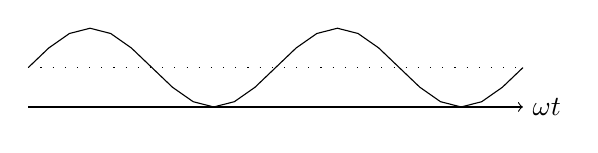
\begin{tikzpicture}
  \begin{scope}[scale=0.5]
    \draw[domain=-2*pi:2*pi]
    plot(\x, {sin(\x r)+1});
    \draw[thin,loosely dotted](-2*pi,1)--(2*pi,1)node[right]{};
    \draw[thin,->](-2*pi,0)--(2*pi,0)node[right]{$\omega t$};
  \end{scope}
\end{tikzpicture}

6-ти пульсная кривая.

\begin{tikzpicture}
  \begin{scope}[scale=1.5]
    \draw[very thin,->] (-pi-0.1,0) -- (pi+0.1,0) node[right] {$\omega t$};
    \draw[thin,->] (-2*pi/3,-0.1)--(-2*pi/3,1.2) node[left] {$U$};
    
  %  \draw[red](-pi,0.65)--(pi,0.65);
  \draw[domain=-pi/2-0.1:pi/2+0.1,help lines,smooth]
  plot(\x, {cos(\x r)});
  \draw[domain=-pi/2+pi/3-0.1:pi/2+pi/3+0.1,help lines,smooth]
  plot(\x, {cos((\x-pi/3) r)});
  \draw[domain=-pi/2-pi/3-0.1:pi/2-pi/3+0.1,help lines,smooth]
  plot(\x, {cos((\x+pi/3) r)});
  \draw[domain=-pi/2+2*pi/3-0.1:pi-pi/4+0.1,help lines,smooth]  
  plot(\x, {cos((\x-2*pi/3) r)});
  \draw[domain=-pi-0.1:-2*pi+pi/2+2*pi/3+0.1,help lines,smooth]
  plot(\x, {cos((\x-2*pi/3) r)});
  \draw[domain=-pi-0.1:pi/2-2*pi/3+0.1,help lines,smooth]  
  plot(\x, {cos((\x+2*pi/3) r)});
%    \draw[domain=2*pi-pi/2-2*pi/3-0.1: pi-pi/4+0.1,help lines,smooth]
%    plot(\x, {cos((\x+2*pi/3) r)});
  \draw[domain=-pi-0.1:-pi/2+0.1,help lines,smooth]  
  plot(\x, {cos((\x+pi) r)});
  \draw[domain=pi/2-0.1:pi-pi/4+0.1,help lines,smooth]
    plot(\x, {cos((\x+pi) r)});
  
  \draw[red] (-pi+0.3-pi/24,0.65)-- (-pi+0.3+pi/24,0.65);
  
  \draw[domain=-pi+0.3+pi/24:-2*pi/3+0.3-pi/6,red,pattern=north east lines,
    pattern color=red]
  (-pi+0.3+pi/24, 0.65) --
  plot(\x, {cos((\x+pi) r)});
  \draw[domain=-pi+0.3+pi/6:-2*pi/3+0.3-pi/24,red,pattern=north east lines,
    pattern color=red]
  plot(\x, {cos((\x+pi) r)})
  -|({-2*pi/3+0.3-pi/24}, 0.65);

  \draw[red] (-2*pi/3+0.3-pi/24,0.65)-- (-2*pi/3+0.3+pi/24,0.65); 

  \draw[domain=-2*pi/3+0.3+pi/24:-pi/3+0.3-pi/6,red,pattern=north east lines,
    pattern color=red]
  (-2*pi/3+0.3+pi/24, 0.65) --
  plot(\x, {cos((\x+2*pi/3) r)});
  \draw[domain=-2*pi/3+0.3+pi/6:-pi/3+0.3-pi/24,red,pattern=north east lines,
    pattern color=red]
  plot(\x, {cos((\x+2*pi/3) r)})
  -|({-pi/3+0.3-pi/24}, 0.65);

 \draw[red] (-pi/3+0.3-pi/24,0.65)-- (-pi/3+0.3+pi/24,0.65);  
  
  \draw[domain=-pi/3+0.3+pi/24:0*pi/3+0.3-pi/6,red,pattern=north east lines,
    pattern color=red]
  (-pi/3+0.3+pi/24, 0.65) --
  plot(\x, {cos((\x+pi/3) r)});
  \draw[domain=-pi/3+0.3+pi/6:0*pi/3+0.3-pi/24,red,pattern=north east lines,
    pattern color=red]
  plot(\x, {cos((\x+pi/3) r)})
  -|({0*pi/3+0.3-pi/24}, 0.65);
  
 \draw[red] (0*pi/3+0.3-pi/24, 0.65)--(0*pi/3+0.3+pi/24, 0.65);
  
  \draw[domain=0*pi/3+0.3+pi/24:pi/3+0.3-pi/6,red,pattern=north east lines,
    pattern color=red]
  (0*pi/3+0.3+pi/24, 0.65) --
  plot(\x, {cos((\x) r)});
  \draw[domain=0*pi/3+0.3+pi/6:pi/3+0.3-pi/24,red,pattern=north east lines,
    pattern color=red]
  plot(\x, {cos((\x) r)})
  -|({pi/3+0.3-pi/24}, 0.65);

 \draw[red] (pi/3+0.3-pi/24,0.65) -- (pi/3+0.3+pi/24,0.65);
  
  \draw[domain=pi/3+0.3+pi/24:2*pi/3+0.3-pi/6,red,pattern=north east lines,
    pattern color=red]
  (pi/3+0.3+pi/24, 0.65) --
  plot(\x, {cos((\x-pi/3) r)});
  \draw[domain=pi/3+0.3+pi/6 : 2*pi/3+0.3-pi/24,red,
    pattern=north east lines,pattern color=red]
  plot(\x, {cos((\x-pi/3) r)})
  -|({2*pi/3+0.3-pi/24}, 0.65);

  % ток
  \draw[thin,->] (-pi-0.1,-1)--(pi+0.1,-1) node[right] {$\omega t$};
  \draw[thin,->] (-2*pi/3,-1.1)--(-2*pi/3,-0.2) node[left] {$I$};
  \draw[red,domain=-pi/3+0.3+pi/24: 0*pi/3+0.3-pi/24]
  plot(\x, {-1-1.5*(\x-(-pi/3+0.3+pi/24))*(\x-(0*pi/3+0.3-pi/24))*(\x-(-pi/2+0.1))});
  \draw[red,domain=0*pi/3+0.3+pi/24: 1*pi/3+0.3-pi/24]
  plot(\x, {-1-1.5*(\x-(0*pi/3+0.3+pi/24))*(\x-(1*pi/3+0.3-pi/24))*(\x-(pi/3-pi/2+0.1))});

  \draw[red,domain=-2*pi/3+0.3+pi/24: -pi/3+0.3-pi/24]
  plot(\x, {-1-1.5*(\x-(-2*pi/3+0.3+pi/24))*(\x-(-pi/3+0.3-pi/24))*(\x-(-pi/3-pi/2+0.1))});

  \draw[red] (-pi/3+0.3-pi/24,-1)--(-pi/3+0.3+pi/24,-1);
  \draw[red] (0*pi/3+0.3-pi/24,-1)--(0*pi/3+0.3+pi/24,-1);
  
  % линии напряжение-ток-\lambda
  \draw[thin] (-pi/3+0.3+pi/24,0.6)-- (-pi/3+0.3+pi/24,-0.95);
  \draw[thin](-pi/3+0.3+pi/24,-1.05)--(-pi/3+0.3+pi/24,-1.4);
  \draw[thin] (0*pi/3+0.3-pi/24,0.3)-- (0*pi/3+0.3-pi/24,-0.95);
  \draw[thin](0*pi/3+0.3-pi/24,-1.05)--(0*pi/3+0.3-pi/24,-1.4);
  \draw[thin,dashed] (-pi/6+0.3+0.03,0.6)--(-pi/6+0.3+0.03,-0.65);
  % lambda
  \draw[thin,<->] (-pi/3+0.3+pi/24,-1.3) -- (0*pi/3+0.3-pi/24,-1.3) node[midway,below]{$\lambda$};  
  \end{scope}  
\end{tikzpicture}  

Знаю, что ток маленький $R_\phi$, $R_D$, $R_\Phi$. $I_\textcyrillic{малое} R_\Sigma$,
много меньше ЭДС синусоиды

$$
\begin{array}{ccc}
  \textcyrillic{ЭДС нагрузки}& + & \xcancel{\textcyrillic{синусоидa}}\\
  \uparrow&&\\
  \textcyrillic{непренебрежимо}
\end{array}
$$

Есть ЭДС нагрузки плюс индуктивность.

$$
e_d -E_\textcyrillic{н} = L_\Sigma \frac{\partial i_d}{\partial t} + \xcancel{i_dR_\Sigma}
$$

Член $i_dR_\Sigma$ демонстративно зачеркнут, потому что второго порядка малости. Даже
при номинальном токе составляет несколько процентов.

$i_d$ это и есть $i_\textcyrillic{фазы}$.

Проинтегрировав эту разность $i_d = f(\omega t)$, а потом возьмём интеграл

$$
I_{d \textcyrillic{среднее}} = \int i_d\; d(\omega t) =
$$

$\displaystyle \lambda = \frac{2\pi}{m}$ -- граничный режим.

$$
\frac{1}{2\pi/m} \int\limits_{-\frac{\pi}{m}+\alpha}^{\frac{\pi}{m}+\alpha}
i_d\;d(\omega t)
$$
-- среднее значение граничного тока.

$$
I_{d\;\textcyrillic{гр}} = f(m,\alpha) = I(\sim)
$$
-- амплитуда пульсаций выпрямленного тока.

Полагая, что $I_\textcyrillic{среднее} =
I_\textcyrillic{амплитуда пульсаций выпрямленного тока}$, получим зависимоть
максимальных пульсаций с учётом гармонического состава. Этот способ учитывает реальную
кривую без разложения её в ряд Фурье.

Чему равна амплитуда тока?
